%Section3.tex

%%%%%%%%%%%%%%%%%%%%%%%%%%%%%%%%%%%%%%%%%%%%%%%%%%%%%%%%%%%%%%%%%%%%%%%%%%%%%%%%%
\section{Real root location}\label{S:three}
%
%
The remaining methods in  \texttt{RealRoots} are linear-algebraic any may be used to cont real zeroes of an ideal $I$ in $\RR^n$ according to
the sign of another polynomial, similar to Sylvester's Theorem~\ref{Th:Sylvester}.
We demonstrate how this may be used for real root location.

A symmetric bilinear form $S$ in a real vector space $A$ has two basic invariants, its rank \defcolor{$\rho(S)$} and signature
\defcolor{$\sigma(S)$}.
If we choose a basis for $A$ and thus a corresponding matrix $M$ representing $S$, then $M$ will be symmetric, and therefore $M$ is
diagonalizable with all $m\vcentcolon = \dim(A)$ eigenvalues real.
The rank $\rho(M)$ of $M$ is its number of nonzero eigenvalues, and its signature  is the difference
\[
\sigma(M)\ \vcentcolon =\ \#\{\mbox{positive eigenvalues of $M$}\}
\ -\ \#\{\mbox{negative eigenvalues of $M$}\}\,.
\]
Sylvester's Law of Inertia asserts that the rank and signature are independent of the choice of basis, and therefore are invariants of the
symmetric form $S$.

Let $I\subset\KK[x_1,\dotsc,x_n]$ be a zero-dimensional ideal of degree $m$ and set $\defcolor{A}\vcentcolon=\KK[x_1,\dotsc,x_n]/I$, an
Artinian ring.
For $f\in A$ (or in $\KK[x_1,\dotsc,x_n]$) multiplication by $f$ induces an endomorphism $m_f$ of $A$ as in Section~\ref{S:two}.
For $h\in A$ (or in $\KK[x_1,\dotsc,x_n]$) we may define the symmetric bilinear \demph{trace form} $S_h$ on $A$ by
$S_h(f,g)\vcentcolon= \mbox{trace}(m_{fgh})$.
The significance of the trace form is the following theorem.

%%%%%%%%%%%%%%%%%%%%%%%%%%%%%%%%%%%%%%%%%%%%%%%%%%%%%%%%%%%%%%%%%%%%%%%%%%%%%%%%%%%%%%%%%%%%%%%%%%%%
\begin{theorem}[\protect{\cite[Thm.\ 4.72]{BPR}}]
  Suppose that $\KK$ is a subfield of $\RR$ and $I\subset\KK[x_1,\dotsc,x_n]$ is a zero-dimensional ideal with zeros
  $\calV(I)\subset\CC^n$.
  For $h\in\KK[x_1,\dotsc,x_n]$, the rank and signature of the trace form $S_h$ satisfy
  %
  \begin{eqnarray*}
    \rho(S_h)&=&
      \#\{ z \in \calV(I) \mid h(z)\neq 0\}   \\
    \sigma(S_h)&=&
        \#\{ z \in \calV(I)\cap\RR \mid h(z)> 0\} \ -\ 
        \#\{ z \in \calV(I)\cap\RR \mid h(z)< 0\} \,.
  \end{eqnarray*}
\end{theorem}
%%%%%%%%%%%%%%%%%%%%%%%%%%%%%%%%%%%%%%%%%%%%%%%%%%%%%%%%%%%%%%%%%%%%%%%%%%%%%%%%%%%%%%%%%%%%%%%%%%%%



(This is for my real root location example and discussion)
\[
\fbox{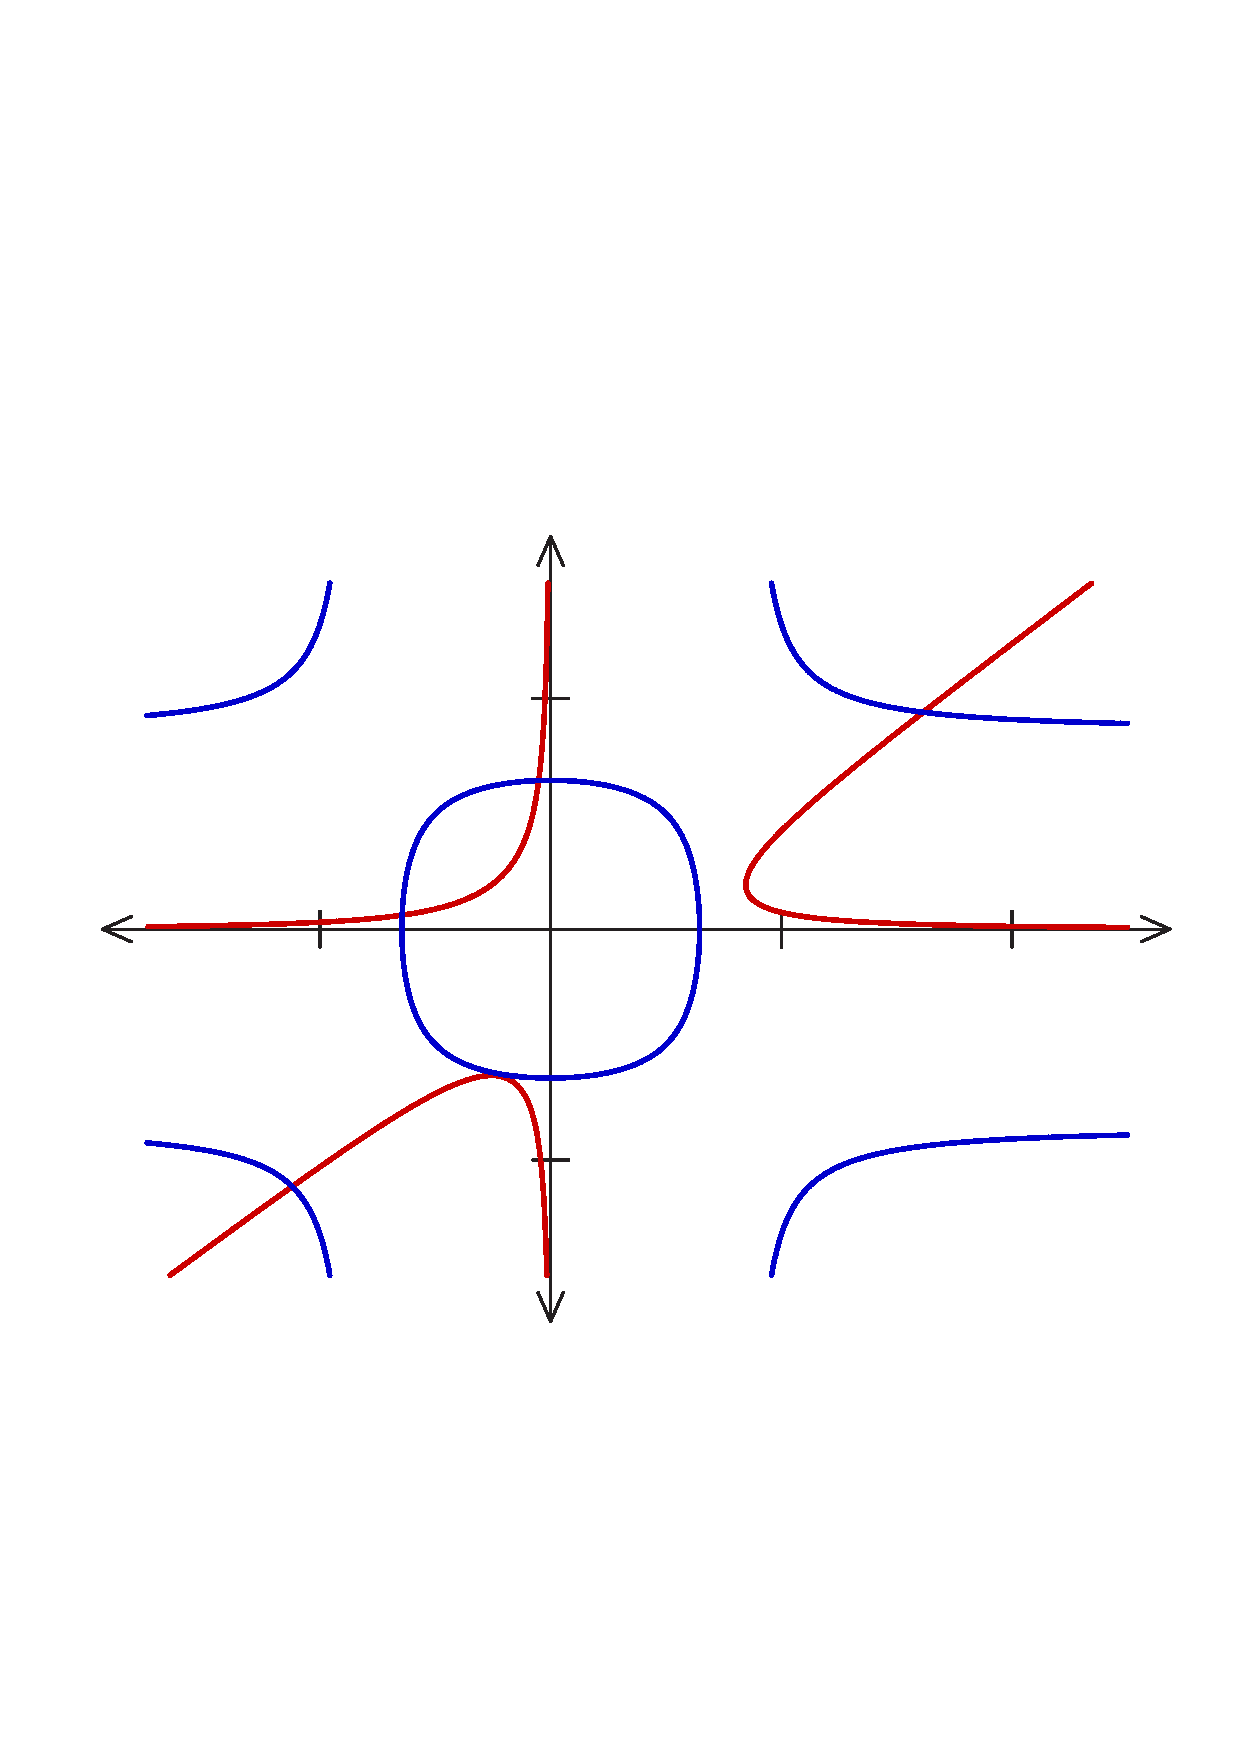
\includegraphics[height=120pt]{pictures/TwoCurves}}
\]
%Trace form is Thm 4.72 in BPR
%
%Sylvester's theorem  is Thm. 2.55 in BPR
%
\newpage
